\documentclass{article}
\usepackage[pdftex]{graphicx}
\graphicspath{{../images/}}
\usepackage{boxedminipage}
\usepackage[hints]{ms}
\usepackage{hyperref}
%\usepackage{ms}
%\usepackage{tikz}
%\usepackage[utf8]{inputenc}
\begin{document}
\begin{titlebox}{White-Dwarf Luminosity Functions}
Ilaria Caiazzo, Jeremy Heyl \\
TAs: Xianfei Zhang, Sarafina Nance, Ilka Petermann
\end{titlebox}

\section{Introduction}

White dwarfs are the final stage in the evolution of stars less than about eight solar masses.  Basically, all nuclear energy generation has ceased, so the stars shrink and cool.  

We have created several models of very young white dwarfs from the evolution of stars of one, two, four and eight solar masses for you to explore the subsequent evolution.

We will look at how white dwarfs move through the Hertzsprung-Russell diagram and colour-magnitude diagrams as they age and also examine the luminosity function of white dwarfs, i.e. how many white dwarfs are there of a given brightness.

\section{The work folder}

In the \texttt{\$MESA\_DIR/star} there is a folder called \texttt{work}. It is provided as a start folder for your projects. For this lab, we took the \texttt{work} folder, renamed it to \texttt{wd\_lab} and made a few changes to the inlists.

For the main inlist, called \texttt{inlist\_project}, we created an inlist very similar to the inlist of the test\_suite directory \texttt{wd\_cool}. It loads a model that we already ran all the way past the end of the AGB and evolves it as it becomes a white dwarf and cools down. The reason why we didn't use the test\_suite \texttt{wd\_cool} in the first place, is because the test\_suite is structured in a way that only the late stages of the white dwarf cooling are saved in the history.data, while we are interested in the entire sequence. Take a look at the inlist to see what type of commands are there.

Also, we used the same \texttt{inlist\_pgstar} as the one we created on the first day, with the difference that instead of a Kipp diagram, now there is a diagram of the total luminosity and the neutrino luminosity vs the age of the star. Feel free to change the \texttt{inlist\_pgstar} to show other interesting properties of the white dwarf as it evolves.

But before starting the run, we need to make some changes.

\textbf{Task:} \\ 
In \texttt{inlist\_project}, the value called \texttt{mesh\_delta\_coeff} is set equal to 2. This parameter determines how fine the mesh is: a larger value increases the max allowed deltas and decreases the number of grid points and a smaller does the opposite. e.g., you will roughly double the number of grid points if you cut \texttt{mesh\_delta\_coeff} in half. We need a high value of \texttt{mesh\_delta\_coeff} in the first few models to help the run relax, but we want a finer mesh for later stages.

Also, the atmosphere boundary condition are set to \texttt{which\_atm\_option = `grey\_and\_kap'}. These are ok for high temperatures, but for effective temperatures lower that 40,000 K, the boundary conditions called \texttt{`WD\_tau\_25\_tables'} are much better for a WD.

We want to use \texttt{run\_star\_extras.f} to make those changes. If you open the file \texttt{src/run\_star\_extras.f}, you'll see that it doesn't contain the usual routines, but it includes the file \texttt{standard\_run\_star\_extras.inc}. This file can be found in the folder \texttt{\$MESA\_DIR/include}.

\begin{enumerate}
    \item Copy the content of \texttt{standard\_run\_star\_extras.inc} into the \texttt{run\_star\_extras.f} file in place of the line \texttt{include `standard\_run\_star\_extras.inc'}. You can see that these are just the standard \texttt{run\_star\_extras} routines. After copying the content into your \texttt{run\_star\_extras.f}, it is safe to try and make your folder to check if you copied everything all right.
    \item Use \texttt{run\_star\_extras.f} to change the \texttt{mesh\_delta\_coeff} to 0.7 after the 15th model.
    \item Use \texttt{run\_star\_extras.f} to change the atmosphere boundary conditions to \texttt{'WD\_tau\_25\_tables'} when the effective temperature falls lower than 40,000 K.
\end{enumerate}

\hint{\textbf{Solution:}\\
\\
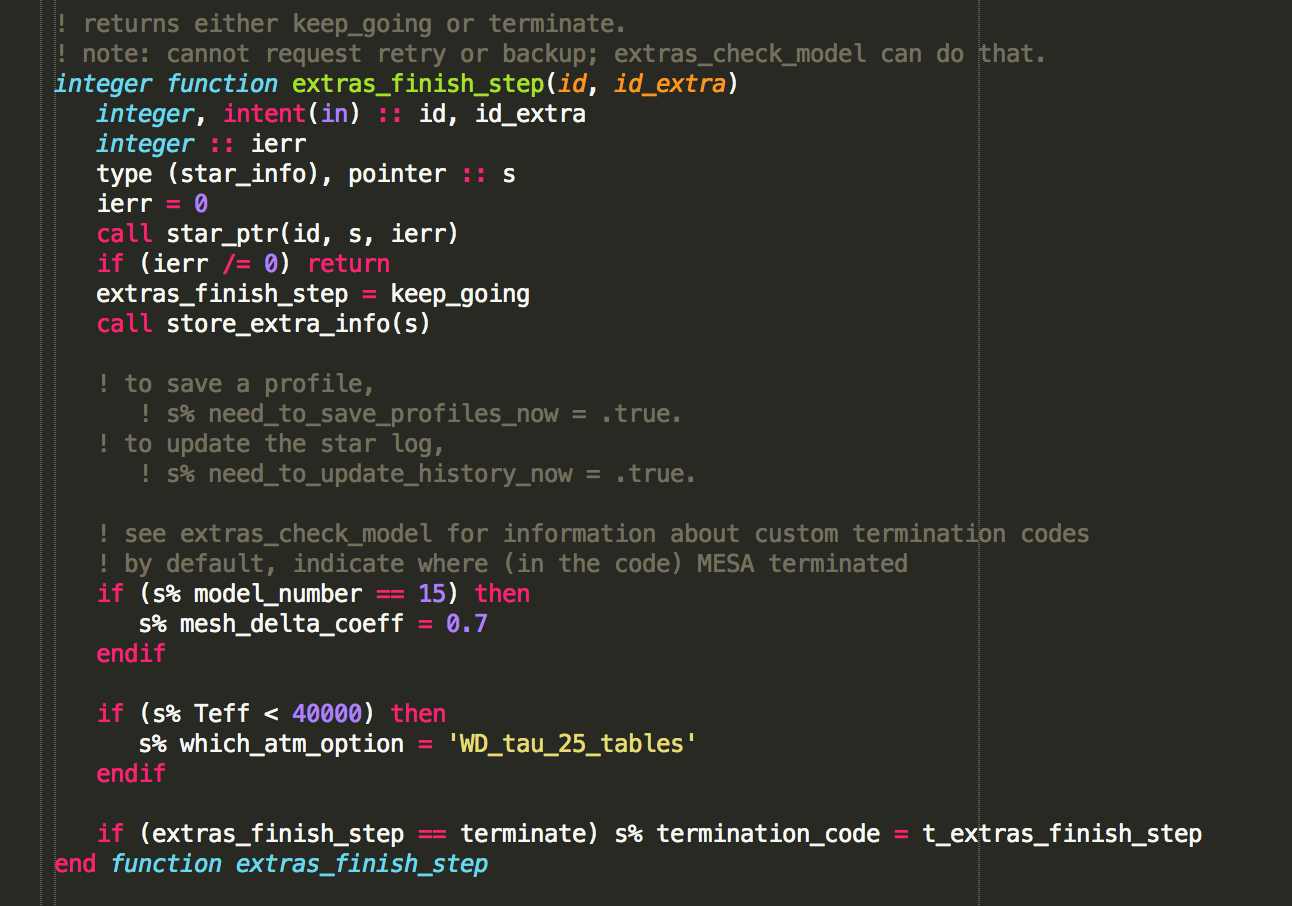
\includegraphics[width=0.8\textwidth]{wd_rse1.png}
}



%We will start with the test\_suite directory wd\_cool and change it for our initial models. 

%\textbf{Task:} \\ 
%Copy the test\_suite directory wd\_cool into your work folder and make the changes needed to use a test\_suite folder outside of its usual environment.

%\hint{\textbf{Hint:}
%You have to remove the \texttt{mesa\_dir = `../../..'} commands %form both the inlists and the makefile.
%}

%You'll see that there are three inlists inside the folder: inlist, inlist\_wd\_cool1 and inlist\_wd\_cool2. That's because the test\_suits wants to run the model with some parameters first, defined in inlist\_wd\_cool1 and, after a while, change to new parameters, defined in inlist\_wd\_cool2.

%\textbf{Task:} \\ 
%Let's understand how this test\_suite works.
%\begin{enumerate}
%    \item First, in which way MESA is switching from one inlist to the other? Look into the \texttt{rn} script to understand how.
%    \item At what moment does the test\_suite do the switch? Look into inlist\_wd\_cool1 and inlist\_wd\_cool2.
%    \item What are the parameters that change from one inlist to the other?
%\end{enumerate}

%If you cannot figure it out, the answers are in the solutions pdf!

%\hint{\textbf{Answers:}
%\begin{enumerate}
%    \item In \texttt{rn}, the routine \texttt{do\_one} is defined, which copies the given inlist into the main inlist, removes the final model if it's already in the folder, and starts the run. This routine is called first for inlist\_wd\_cool1 and then for inlist\_wd\_cool2.
    
%    So this is what happens:
%    \begin{itemize}
%        \item \texttt{rn} first copies inlist\_wd\_cool1 into the main inlist, removes the model `hires\_surface.mod' (if it exists already) and starts the run.
%        \item When the run stops, it will have produced the model `hires\_surface.mod'.
%        \item At that point, \texttt{rn} copies inlist\_wd\_cool2 into the main inlist, removes the model 'final.mod' (if it exists already) and starts the run.
%        \item This time, the run will load the model `hires\_surface.mod' previously produced as its first model and it will produce the model 'final.mod'.
%    \end{itemize}
%    \item MESA will switch between the two inlists when the first run terminates. If you look into inlist\_wd\_cool1 you'll see that this happens when it reaches a maximum model number of 31.
%    \item The main difference is that the first inlist uses an atmosphere boundary condition called \texttt{grey\_and\_kap} and the second one the one called \texttt{WD\_tau\_25\_tables}. Also, the second inlist turns up the spatial resolution (\texttt{mesh\_delta\_coeff = 0.7}).
%\end{enumerate}

%}

%Now that you understand how this test\_suite works, let's make some changes. The first inlist loads a model that is already past the end of the AGB and on its way to be a WD. In the folder, we provided you with other similar starting models that have different masses.

%\textbf{Task:} \\ 
%Change the line with saved\_model\_name to use our first model from a one-solar-mass star (\texttt{52SMWD.mod}).  We will look at the other white dwarfs a bit later. We also want to make more changes to the inlist in order to adapt it to our needs.
%\begin{enumerate}
%    \item The first inlist saves a model at model\_number 31 and then stops the run at model number 32. The \texttt{52SMWD.mod} model starts at \texttt{model\_number = 7131}, so you might want to reset the model\_number or the star\_age using the following commands:
%    \begin{verbatim}
%        &star_job
%        set_initial_model_number = .true.
%        initial_model_number = 0
%        set_initial_age = .true.
%        initial_age = 0
%    \end{verbatim}
%    \item Change the second inlist's stopping condition on luminosity to let the run go until \texttt{log\_L} $ < -4$ (instead of -1).
%    \item The second inlist has also a stopping condition on \texttt{model\_number} which might prevent your run to go all the way to \texttt{log\_L} $ < -4$. In that case, comment out the corresponding command or increase the maximum model number.
%\end{enumerate}

\section{The Evolution}

As the \texttt{52SMWD.mod} runs, take a look at the Jupyter notebook called White-Dwarf-Lab. A few example plots are shown for a history.data file that comes from the evolution of a more massive WD ($M=1.17$ M$_\odot$).

\textbf{Task:}\vspace{-1em}
\begin{enumerate}
 \setlength\itemsep{0em}
\item Let's first look at the track of luminosity against effective temperature.  What is happening to the star?
\item Let's look at luminosity against core temperature.  What is happening here?  What are the different regimes?
\item Let's look at luminosity against time.  What are the different regimes here?
\item When the run for \texttt{52SMWD.mod} stops, try loading its history.data file in the notebook and add its curves to the plots. This model is for a white dwarf that results from a one-solar-mass star.  This is typical for the white dwarfs in globular clusters. What are the differences?
\item If you have time, try running the evolution for a more massive white dwarf and add their curves to the preceding diagrams.
\end{enumerate}

\hint{
\textbf{Hint:}

You may find that some of the models fail to run.  You can try increasing the number of retries and backups or changing the \texttt{varcontrol} parameter.

}

%\textbf{Bonus Task:}\\
%You can use the include program \texttt{makefakehistory.py} to recalculate the thermal evolution assuming that specific heat capacity of the star is constant (it remains liquid) or that the cooling is due to emission of radiation from the surface.  Compare the results of these simulations to the original ones.

\section{Observations}

\subsection{The outer field}
We have included a file with the observed fluxes of about 2,000 old white dwarfs in the globular cluster 47 Tucanae.  The white dwarfs that are being born in this cluster come from stars whose masses are just a bit less than the mass of the Sun.   Because the white dwarfs are relatively young compared to the age of the cluster, we can assume that they are being born at a constant rate, so their cumulative luminosity function is an estimate of their cooling evolution.

The file with the observed white dwarfs is called \texttt{47tuc\_fromIR.dat} and presents the observed magnitudes in the Hubble filters F814W (second column) and F606W (third column), and the difference between the two (first column).

\textbf{Task: Old White Dwarfs}\vspace{-1em}
\begin{enumerate}
 \setlength\itemsep{0em}
\item Use the \texttt{paintisochrone.py} program to add absolute magnitudes to your history files.  We have provided an atmosphere file for this called \texttt{colmag.Bergeron.all.Vega.txt}. The code needs three arguments, the name of the history file, the name of the atmosphere file, and the name of the output file. In the Jupyter notebook you can see the example we made for the history\_example.data file that we provided.
\item Plot the colour $F814W$ against $F606W-F814W$ from your models
\item Plot $F814W$ against time.
\end{enumerate}

Now that we have the magnitudes in 814 and 606, we can finally compare our models with observations.

\textbf{Task:}\vspace{-1em}
\begin{enumerate}
\item Load the file \texttt{47tuc\_fromIR.dat}.
\item Make a CMD plotting the colour $F814W$ against $F606W-F814W$ from the data. This is the WD cooling sequence of 47 Tucanae.
\item Add both theoretical curves on the plot: the one called \texttt{paintedhistory\_ex.data} and the one you made. And others if you made more than one.
\item You can see that both of them fall far from the data. That's because the models are still in absolute magnetudes, while the data is in observed magnitudes. In order to compare them, we need to add the distant modulus (13.45) and reddening (0.065) to the models, for example:
\begin{verbatim}
    plt.plot(pdata['F606W']-pdata['F814W']+0.065,pdata['F814W']+13.45,c='r')
\end{verbatim}
\item Now we can compare them. Which evolution does the data agree with the best?
\end{enumerate}

If we assume that the white dwarfs in the cluster are born at a constant rate, we can use their cumulative luminosity function as a proxy for their cooling evolution. In the file \texttt{47tuc\_fromIR.dat} there is a column called `cumweight', that indicates, for each star, how many stars we expect in the field at that magnitude or brighter.  This cumulative distribution is calculated by counting how many stars are in the image and correcting the number for the ones that the telescope might have missed (the completeness is given as a percentage in the column `comp'. In this field, which is in the outskirts of the cluster, we estimated the birth rate to be about 1 WD every $6 \times 10^6$ years.

\textbf{Task:}\vspace{-1em}
\begin{enumerate}
\item Plot the magnitude in $F814W$ against the cumulative distribution divided by the birth rate (you can just multiply `cumweight' by $6 \times 10^6$~years). You will get the cooling curve of the white dwarfs in the cluster. Make the x-axis logarithmic.
\item On top of it, plot the magnitude in $F814W$ against the log of the star age for your theoretical models. And don't forget to add the distance modulus!
\item Since the zero age of the WD we chose is arbitrary, you might have to add or subtract some small constant to the age of your models to make them fit better the data. 
\item Which evolution does the data agree with the best?
\end{enumerate}

\textbf{Bonus Task:}\\
If one of your white dwarf evolutions lasted long enough, you will see the effects of the onset of convection in the cooling track.  Compare this model with observations.   Plot the profile files that correspond to when the bump in the cooling curve occurs to verify that both convection and freezing are occurring.   Perhaps add entropy information to the profile and re-run. 

\hint{\textbf{Hint:}

The key parameter to plot is the specific entropy but it doesn't get output in the profile file by default.  You could add it and restart your run using the \texttt{re} command with a photo file or you could plot $\log P$ against $\log \rho$.

}

\subsection{The inner field}

In the file \texttt{47tuc\_fromUV.dat} you can find the observed flux from about 3000 white dwarfs. These white dwarfs live in the center of the cluster, where the density of stars is extremely high. For this reason, it is hard to detect white dwarfs in the visible or in the infrared, as the light is dominated by the very bright red giants. However, young white dwarfs are the brightest objects in the UV, because they are very hot. That's why we observed them in the filters $F225W$ and $F336W$ with Hubble. You can see the UV image here: \url{http://coolpulsars.org/images/47TucCore_Image/}.  The white dwarfs are the blue dots.

This set of young white dwarfs in the UV is what we are going to use in the next lab, so let's take a look at it.

\textbf{Task: Young White Dwarfs}\vspace{-1em}
\begin{enumerate}
 \setlength\itemsep{0em}
\item Make a CMD with the magnitude $F225W$ against $F225W-F336W$ from the data and from your models. The distance modulus is of course the same, but do you need to add reddening in these filters? How much?
\item Make a cumulative distribution plot for $F225W$ as we did before for $F814W$. This time though, since we are in the center of the clusters and the density of stars is higher, we expect a higher birth rate. Can you figure it out from comparing the models with the data?
\end{enumerate}

We will study the young white dwarfs in more detail in the next lab where you will program MESA to vary the neutrino rates within the white dwarfs and see what happens.

\end{document}
